%!Mode:: "TeX:UTF-8"
 
\section{缓存}
\cite{wikipedia}:

\subsection{CPU高速缓存结构}
m位地址,有$m=t+s+b$, 寻址空间$M=2^m$, 缓存容量$C=S \times E \times B=2^s E 2^b$, $C<M$则$E < 2^t$.

直接相连:$E=1$.
全相连:$S=1$.


\begin{figure}[ht]
	\begin{center}
	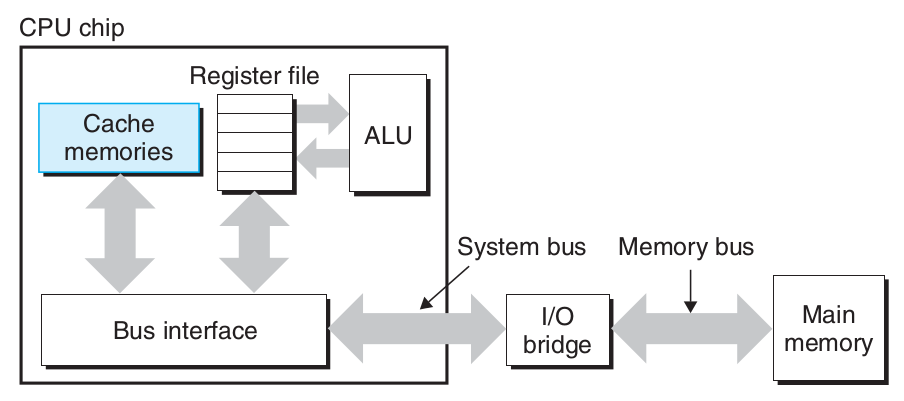
\includegraphics[keepaspectratio,width=0.3\paperwidth]{Pictures/cacheBus.png}
		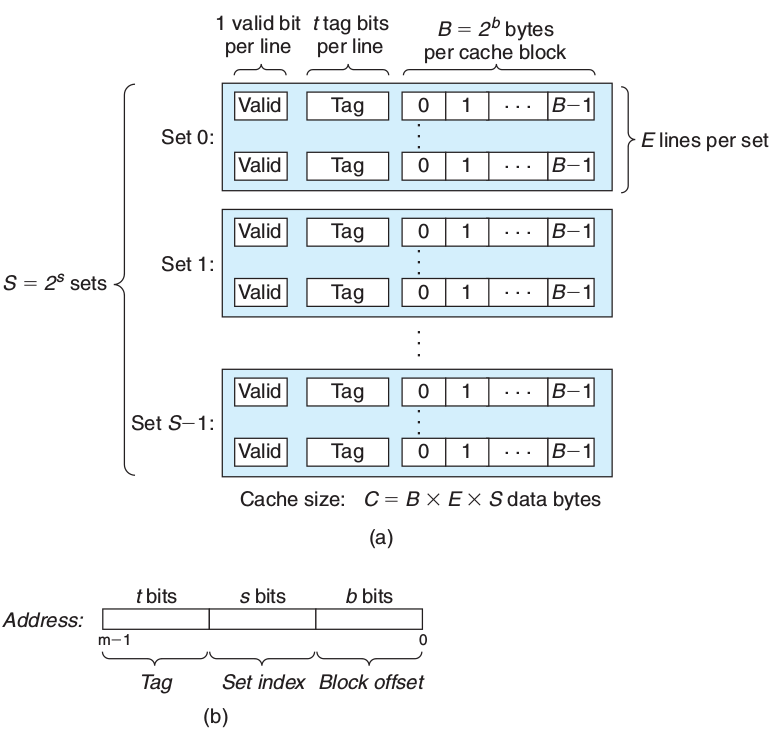
\includegraphics[keepaspectratio,width=0.3\paperwidth]{Pictures/cache.png}
	\caption{高速缓存通用结构}
	\label{fig:cacheMemStructure}
	\end{center}
\end{figure}


\subsection{TLB}
分页表是一种数据结构,用于计算机操作系统中的虚拟内存系统,存储了虚拟地址到物理地址间的映射。虚拟地址在访问进程中是唯一的,物理地址在硬件中是唯一的。比如RAM。CPU的内存管理单元(memory management unit MMU)存储最近用过的映射缓存,来自操作系统分页表。被称为转译后备缓冲器(translation lookaside buffer, TLB)。TLB是一个索引缓存。

转译后备缓冲器(英文:Translation Lookaside Buffer,首字母缩略字:TLB),在中国大陆也被翻译为页表缓存、转址旁路缓存,为CPU的一种缓存,由存储器管理单元用于改进虚拟地址到物理地址的转译速度。目前所有的桌面型及服务器型处理器(如 x86)皆使用TLB。TLB具有固定数目的空间槽,用于存放将虚拟地址映射至物理地址的标签页表条目。为典型的内容可寻址存储器(content-addressable memory,首字母缩略字:CAM)。其搜索关键字为虚拟内存地址,其搜索结果为物理地址。如果请求的虚拟地址在TLB中存在,CAM 将给出一个非常快速的匹配结果,之后就可以使用得到的物理地址访问存储器。如果请求的虚拟地址不在 TLB 中,就会使用标签页表进行虚实地址转换,而标签页表的访问速度比TLB慢很多。有些系统允许标签页表被交换到次级存储器,那么虚实地址转换可能要花非常长的时间。

在任务(task)切换时,部分 TLB 条目可能会失效,例如先前运行的进程已访问过一个页面,但是将要执行的进程尚未访问此页面。最简单的策略是清出整个 TLB。

多核系统的每个核都有自己的TLB。与cache不同,TLB不需要核间同步,因为每个核运行的进程有不同的地址映射。


\subsection{缓存一致性}
分布式共享内存(Distributed Shared Memory,DSM)指物理上分布式的内存可以在逻辑上被当做一块内存来访问。这里的共享指的是地址空间的共享。
为维护“内存一致性”(memory coherence),需选择一个“一致性协议”(coherence protocol)来实现一种"一致性模型"(consistency model)。
DSM系统的实例包括OpenSSI,MOSIX,Kerrighed,TreadMarks等。注意同“分布式缓存”区分开。

\begin{quotation}
分布式缓存(Distributed cache)是对传统意义上单点缓存概念的扩展,使得缓存可以跨越多个服务器。
由于主存变得便宜,以及网卡速度的增强,分布式缓存得以变得现实。
分布式缓存的例子包括:Oracle Coherence, Ehcache, Hazelcast, Memcached, SafePeak, Riak, Redis等。
\end{quotation}

在多核系统下也存在内存一致性问题。
如果多核同时访问同一共享内存区,且存在写操作,就可能出现缓存一致性(内存一致性)问题,即某核读到的本地缓存副本不是最新的。
需要引入“内存一致性协议”(memory coherence protocol)来解决这个问题。

一致性的实现方式包括:
\begin{description}
\item[基于目录的实现(Directory-based)]目录维护各缓存间的一致性信息。处理器在将内存值加载到本地cache时时必须先查询目录。
当某一表项被更新时,目录要么标记其失效,要么主动更新所有其他缓存。
\item[Snooping]每一个本地cache监控地址线,如果一个内存更新访问涉及自己所缓存的对象,那么本地缓存的这个副本应被失效。
\end{description}
这些实现机制可用于多核、多处理器缓存,以及分布式共享内存系统。

一致性模型"(consistency model)包括:
\begin{description}
\item[线性一致性(Linearizability)]或严格一致性(Strict consistancy)、原子一致性(Atomic consistancy):任何对一个内存位置X的读操作,将返回最近一次对该内存位置的写操作所写入的值。
\item[顺序一致性(sequential consistency)](并发程序在多处理器上的)任何一次执行结果都相同,就像所有处理器的操作按照某个顺序执行,各个微处理器的操作按照其程序指定的顺序进行。
换句话说,所有的处理器以相同的顺序看到所有的修改。读操作未必能及时得到此前其他处理器对同一数据的写更新。但是各处理器读到的该数据的不同值的顺序是一致的。
\item[释放一致性(Release consistency )]
同步操作被分裂成获得(acquire)和释放(release)操作。
如果某进程的写操作在该进程执行释放之后、在其他进程执行获取之前被看到,则称释放一致性。
释放一致性可以通过两种一致性协议来实现:
一致性操作(coherence actions)可以在退出临界区时完成(渴望释放一致性),也可推迟到下一次进入临界区(懒惰释放一致性)。
\item[因果一致性(Causal consistency )]
因果一致的存储器应遵守以下条件:可能因果相关的写操作应对所有进程可见,且顺序一致。并发写操作在不同机器看来顺序可能是不同的。
如果进程A通知进程B它已更新了一个数据项,那么进程B的后续访问将返回更新后的值,且一次写入将保证取代前一次写入。与进程A无因果关系的进程C的访问遵守一般的最终一致性规则。因果一致性弱于顺序一致性,强于PRAM一致性。
假设进程P1写变量x,然后P2读出x,写入y。这里读出x和写入y之间可能有潜在的因果联系,因为y的计算很可能决定于P2读到的x值(即P1写入的值)。 另一方面,若两进程自然而同时地写两个变量,就没有因果联系。先有读操作之后执行写操作,两个事件就可能有因果联系。相似的,读和提供所读数据的写有因果关系。没有因果关系的操作称为并发的(concurrent)。
\item[PRAM(Piplined RAM)一致性]又称FIFO一致性,几乎等同于处理机一致性(Processor consistency)。
一个进程(处理机)的多个写操作被另一进程按照相同的顺序接收到,如同在流水线中到达一样,但来自多个进程的写操作顺序不定。PRAM一致性很容易实现。
对于双处理器,处理器一致性与顺序一致性是等价的。
\item[Delta一致性]在固定时间Delta之内达到全局一致。
\item[弱一致性]弱一致性有三个属性:a. 对同步变量的访问是顺序一致的;
b. 在所有先前的写操作完成之前,不能访问同步变量;
c. 在先前所有同步变量的访问完成前,不能访问(读或写)数据。
\end{description}













\clearpage